\section{Durchführung}

    Der folgende Abschnitt stellt die verwendete Messapparatur vor.
    Zudem wird beschrieben,
    wie das Emissions- und Absorptionsspektrum
    sowie die Bragg-Bedingung gemessen werden.


\subsection{Versuchsaufbau}

    \begin{figure}
        \centering
        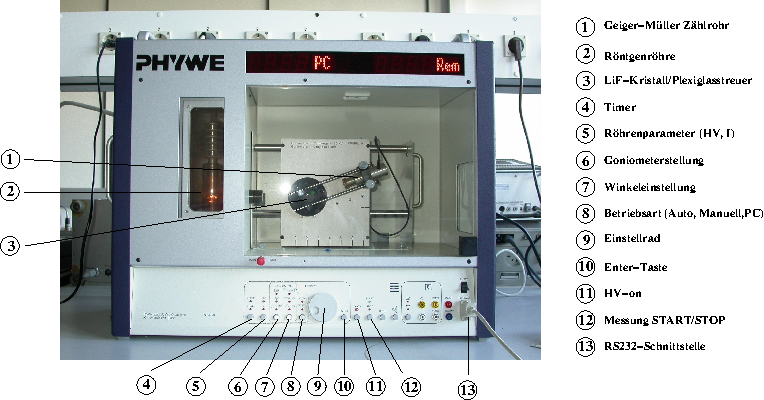
\includegraphics[width=\textwidth]{content/img/Abb_4_compressed.pdf}
        \caption{Die Versuchsapparatur mit Benennung der Bestandteile. \cite{versuchsanleitung}}
        \label{fig:Versuchsapparatur}
    \end{figure}

    In \autoref{fig:Versuchsapparatur} ist die gesamte Versuchsapparatur dargestellt.
    Die Hauptbestandteile sind eine Kupfer-Röntgenröhre,
    ein LiF-Kristall,
    der für die Bragg-Reflexion verwendet wird,
    und ein Geiger-Müller-Zählrohr.
    Die Röntgenröhre ist auf den Kristall ausgerichtet,
    wobei dieser gedreht werden kann,
    um die Intensität der Röntgenstrahlung mithilfe des Geiger-Müller-Zählrohrs für verschiedene Glanzwinkel zu messen.
    Die Messung kann mithilfe der Einstellelemente im unteren Bereich der Apparatur geregelt werden.
    Für alle Messungen wird eine Beschleunigungsspannung von $U_\text{B} = \SI{35}{\kilo\volt}$ an der Röntgenröhre eingestellt,
    sowie ein Emissionsstrom von $I = \SI{1}{\milli\ampere}$ am Geiger-Müller-Zählrohr.
    Mithilfe der Winkeleinstellung \textbf{7} kann ein fester Winkel des LiF-Kristalls eingestellt werden.
    Zudem muss darauf geachtet werden,
    dass die $\SI{1}{\milli\meter}$-Blende und der Kristall in den jeweiligen Halterungen sind.
    Die Schlitzblende muss in Drehrichtung waagerecht auf dem Geiger-Müller-Zählrohr angebracht sein.
    %Warum waagerecht????
    \\
    Die Messergebnisse können über einen Rechner aufgenommen werden;
    dazu wird unter dem Programmpunkt \textit{measure} unter \textit{Messgeräte} das Röntgengerät ausgewählt.
    Es können die Messart, der Drehwinkel $\theta$, ein Drehmodus und eine Integrationszeit $\symup{\Delta}t$ festgelegt werden.
    Die Messart muss dabei auf \textit{Spektren} eingestellt sein.


\subsection{Überprüfung der Bragg-Bedingung}

    Für diese Messung wird am Rechner das Programm \textit{2:1 Koppelmodus} ausgewählt.
    Für die Überprüfung der Bragg-Bedingung wird der LiF-Kristall auf einen festen Winkel von $\theta = \SI{14}{\degree}$ eingestellt.
    Mit einem Winkelzuwachs von $\symup{\Delta}\theta = \SI{0.1}{\degree}$ in einer Integrationszeit von $\symup{\Delta}t = \SI{5}{\second}$
    wird die Intensität der Röntgenstrahlung am Geiger-Müller-Zählrohr in einem Winkelbereich von $\theta_\text{GM} = \SI{26}{\degree}$
    bis $\theta_\text{GM} = \SI{30}{\degree}$ gemessen.


\subsection{Das Emissionsspektrum der Kupfer-Röntgenröhre}

    % Für diese Messung wird am Rechner das Programm [TODO] ausgewählt.
    Es wird in einem Winkelbereich von $\theta = \SI{8}{\degree}$ bis $\theta = \SI{25}{\degree}$ in Schritten von $\symup{\Delta}\theta = \SI{0.1}{\degree}$ gemessen.
    Als Integrationszeit wird $\symup{\Delta}t = \SI{10}{\second}$ gewählt.
    Das Röntgenspektrum wird in einer Beugungsordnung von $n=1$ ausgemessen.
    \\
    Das Auflösungsvermögen wird
    %mithilfe von \autoref{eqn:Auflösungsvermögen} %%Theorie l.91-97
    bestimmt,
    wobei die Halbwertsbreiten gemessen werden.

    Mithilfe der Gleichungen \eqref{eqn:EnergieKalpha} und \eqref{eqn:EnergieKbeta} können die Abschirmkonstanten $\sigma_1$, $\sigma_2$, und $\sigma_3$, bestimmt werden,
    wobei $m=2$ und $l=3$ zu wählen sind.

    \begin{align}
    \begin{split}
        \label{eqn:sigma_123}
        \sigma_1 &= Z -   \sqrt{\frac{E_\text{K,abs}}{R_\infty}} \\
        \sigma_2 &= Z - 2 \sqrt{\frac{1}{n^2} (Z - \sigma_1)^2-\frac{E_{K,\alpha}}{R_\infty}} \\
        \sigma_3 &= Z - 3 \sqrt{\frac{1}{n^2} (Z - \sigma_1)^2-\frac{E_{K,\beta}}{R_\infty}} \; .
    \end{split}
    \end{align}


\subsection{Das Absorptionsspektrum verschiedener Materialien}

    Um das Absorptionsspektrum zu messen,
    wird ein Absorber zwischen dem LiF-Kristall und dem Geiger-Müller-Zählrohr angebracht,
    sodass die Röntgenstrahlung nach der Reflexion auf den Absorber und nicht direkt auf das Zählrohr trifft.
    Das Absorptionsspektrum wird in Abständen von $\symup{\Delta}\theta = \SI{0.1}{\degree}$ mit einer Integrationszeit von $\symup{\Delta}t = \SI{20}{\second}$ gemessen.
    Die Winkelbereiche werden für jedes Material einzeln gewählt.
    Als Absorber dienen Materialien mit Ordnungszahlen von $30 \leq Z \leq 50$.
    Hier sind es Zink, Gallium, Brom, Rubidium, Strontium und Zirkonium,
    deren Literaturwerte in \autoref{sec:vorbereitung} angegeben sind.
    Mithilfe der Gleichungen \eqref{eqn:EnergieKalpha} und \eqref{eqn:EnergieKbeta} und der Literaturwerte können die Abschirmkonstanten berechnet werden.
    Die Rydbergenergie $R_\infty = R \cdot h$ kann nach dem Moseley'schen Gesetz mit \autoref{eqn:Moseley} bestimmt werden.
